\documentclass{article}

\usepackage[utf8]{inputenc}
\usepackage[spanish, mexico]{babel}
\usepackage[export]{adjustbox}
\usepackage{hyperref, amsmath, xcolor, mdframed, listings, tikz, enumitem}
\usetikzlibrary{shapes, arrows, chains, fit, calc} 

\usepackage{showframe}


\newcommand{\crule}[2][1pt]
    {\begin{center}\rule{#2\textwidth}{#1}\end{center}}

\newcommand{\red}[1]	    {\textcolor{red}{#1}}


\newcommand\refcode[2]{ \href{#1}{\texttt{#2}} }

\newenvironment{note}
    {\begin{mdframed}[leftmargin=1cm, 
                 skipabove=1em,
                 skipbelow=1em,
                 rightline=false, 
                 topline=false,
                 bottomline=false,
                 linewidth=2pt]
        \textbf{Nota}\\}
    {\end{mdframed}}
    

% http://tex.stackexchange.com/questions/68547/alignment-across-nested-aligned-environments
%\newlength{\myleftlen}
%\newcommand{\setmyleftlen}[1]{\settowidth{\myleftlen}{\( \displaystyle#1\)}}
%\newcommand{\backup}{\hskip-\myleftlen\mkern-7mu}



\title{ \includegraphics[scale=0.6, right]{itesm_logo}
	    \\[4em] 
        Sistemas Conexionistas y Evolutivos
        \\[2em]
        $1^\text{er}$ parcial: reporte % babel shorthands don't work in macros.
        \\[1em]
        }
\author{ \vspace*{\fill} \red{ Personal Data} \qquad\small \red{Axxxxxxxx} \\[1em] }

\date{ \vspace*{\fill} \today, Puebla.}


\begin{document}
\lstset{language=Haskell, frame=single, 
    keywordstyle=\color{blue}, 
    deletekeywords={min,max},
    otherkeywords={N8}
    }

\maketitle
\newpage

\def\ImgCharRoot{run:./docs/image-characteristics}
\def\ImgCharacteristics{\ImgCharRoot/ImgCharacteristics.html}
\def\Friday{\ImgCharRoot/ImgCharacteristics-Friday.html}
\def\Extractors{\ImgCharRoot/ImgCharacteristics-Friday-Extractors.html}
\def\ExtractorBuilder{\ImgCharRoot/ImgCharacteristics-ExtractorBuilder.html}
\def\GTK{\ImgCharRoot/ImgCharacteristics-GTK.html}
\def\Weka{\ImgCharRoot/ImgCharacteristics-Weka.html}

\def\ExecAll{run:./docs/image-characteristics/img-chv_descriptive-stats_all/src/Main.html}

\def\Nat{run:./docs/Nat/frames.html}
\def\WekaData{run:./docs/WekaData/frames.html}

\section{Base de imágenes}

Se seleccionaron 42 imágenes de bosques \underline{con resoluciones diferentes}, 36 de las cuales contienen incendios forestales. Seis mas no contienen ningún signo de fuego, y tres de ellas presentan un bosque en otoño con las hojas de color. Las imágenes se adjuntan en archivo \textit{images.zip}.

\begin{note}
La partición de imágenes en regiones se adapta al tamaño de la imagen, lo que permite recibir regiones con desviaciones de tamaño reducidas. Ademas, el vector de características se forma por los valores estadísticos de la región, los cuales no están afectados por la diferencia en el tamaño de la muestra.
\end{note}


\section{Partición de imágenes}

El proceso de partición es parte de la aplicación \verb|image-characteristics|, la cual se discute mas detalladamente en la siguiente sección.

Esta representado por un \href{http://learnyouahaskell.com/types-and-typeclasses}{\emph{clase de tipos}} \verb|RegionsExtractor| en el archivo 
\refcode{\ImgCharacteristics}{src/ImgCharacteristics.hs}.
Al momento tiene una implementación para \verb|FixedColRowRegions|, el cual describe:
\begin{enumerate}
\item el número de filas deseado (el número máximo);
\item el número de columnas deseado (el número máximo);
\item el tamaño mínimo de un \emph{región}.
\end{enumerate}

La implementación se llama \verb|fixedColRowRegions| y se encuentra en\\ \refcode{\Friday}{src/ImgCharacteristics/Friday.hs}. Utiliza la función \verb|finalSize| para encontrar el número máximo de columnas y filas, que producirán regiones de tamaño no menor al establecido por \verb|FixedColRowRegions|. La partición de la imagen se hace con la función \href{https://hackage.haskell.org/package/friday-0.2.2.0/docs/Vision-Image-Transform.html}{\emph{crop}} de la librería \verb|friday|.

Se espera la declaración de una \href{https://downloads.haskell.org/~ghc/7.0.1/docs/html/users_guide/type-class-extensions.html}{\emph{instancia}} de \verb|RegionsExtractor| en el modulo \verb|Main|, cómo en \refcode{\ExecAll}{exec/DescriptiveStatsAll.hs} (está diseñado de esta manera para evitar posibles \href{https://wiki.haskell.org/Multiple_instances}{conflictos} de importación).

\section{Vector de características}

Un vector de características se extrae de una región de imagen por las clases \verb|CharacteristicExtractor| y \verb|CharacteristicExtractors|, los cuales definen los extractores y sus nombres. Están basados en vectores, indexados con \href{https://wiki.haskell.org/Type_arithmetic}{\emph{números naturales en nivel de tipos}}, implementados en el proyecto \refcode{\Nat}{Nat}.

Los extractores mencionados se construían utilizando \verb|ChanelExtractor| y \verb|LinkedChanelExtractor|, definidos en \\ \refcode{\ExtractorBuilder}{src/ImgCharacteristics/ExtractorBuilder.hs}.


Para el problema dado se utilizan los siguientes extractores de canales, definidos en \refcode{\Extractors}{src/ImgCharacteristics/Friday/Extractors.hs}:
\begin{itemize}
\item \verb|mean| --- la esperanza matemática;
\item \verb|meanQuadratic| --- la media cuadrática, $\sqrt{\frac{\sum\limits_{i=1}^n x_i^2}{n}}$;
\item \verb|stdev'| --- la desviación estándar, requiere valor de la media;
\item \verb|min| --- el valor mínimo ($Q_0$);
\item \verb|max| --- el valor máximo ($Q_5$);
\item \verb|quartiles| --- los cuartiles $Q_1, Q_2, Q_3$;
\end{itemize}

En total son \textbf{8} características. \\

\noindent Los extractores de canales se aplican a cada canal de la región (independientemente). Un vector de características tiene dimensión \emph{número de características} $\times$ \emph{número de canales}.

\medskip

\noindent Definición de \verb|ChanelExtractor| utilizado:
\begin{lstlisting}
import ImgCharacteristics.Friday.Extractors as CE

descriptiveStats :: ( NatRules n, Floating num
                    , Ord num, GenVec n
                    , NatRules3Pack n
                    ) => ChanelExtractor n num N8
descriptiveStats =    CE.min
                  +#  CE.quartiles
                  +#  CE.max
                  +#  CE.meanQuadratic
                  +## CE.meanAndVar
\end{lstlisting}

\medskip

Para transformar \verb|ChanelExtractor| a \verb|CharacteristicsExtractor| se utilizan las funciones \verb|extractorRGB|, \verb|extractorHSV| y \verb|extractorGrey|.

Se encuentran en \refcode{\Friday}{src/ImgCharacteristics/Friday.hs}.\\

En el ejecutable utilizado (\refcode{\ExecAll}{exec/DescriptiveStatsAll.hs}) se combinan los extractores \verb|RGB, HSV, Grey| para recibir vectores de dimensión \emph{56} ($8\times3 + 8\times3 + 8\times1$).

\section{Datos de aprendizaje}

Para el aprendizaje \emph{supervisado}, se requieren las etiquetas de clase para cada instancia de los datos. El funcionamiento de selección de etiquetas está definido por la clase \verb|RegionsClassesProvider| (en \refcode{\ImgCharacteristics}{src/ImgCharacteristics.hs}) y está diseñado para una acción de \href{https://www.haskell.org/tutorial/io.html}{\emph{entrada/salida}}. Provee dos funciones:
\begin{enumerate}
    \item \verb|classProvider| --- crea una instancia de \verb|RegionsClassesProvider|;
    \item \verb|regionClass| --- pregunta la clase de la imagen (región).
\end{enumerate}

Específicamente, está implementado a través de ``GIMP Toolkit'' (GTK), el cual se utiliza para la interfaz gráfica ``GNOME''. La interfaz de la ventana está proveída por un contenedor \verb|ClassesInterview|, definido en \\ \refcode{\GTK}{src/ImgCharacteristics/GTK.hs}, el cual provee:
\begin{itemize}
    \item \verb|ciWindow| --- el objeto de la ventana gráfica;
    \item \verb|ciAskClass| --- una función \verb|a -> IO class'|, dónde \verb|a| es una 
                                imagen (una región);
    \item \verb|ciDestroy| --- una función para destruir la interfaz gráfica.
\end{itemize}

\crule{1}
\medskip
Creación del \verb|ClassesInterview|:
\medskip

% see http://www.texample.net/tikz/examples/flexible-flow-chart/

\begin{tikzpicture}[%
    >=triangle 60,              % Nice arrows; your taste may be different
    node distance=20mm and 50mm, % Global setup of box spacing
    ]

\def\bind{$>>=$}

\tikzset{
  base/.style={draw, on grid, align=center, minimum height=4ex,text width=8em}, % on chain, 
  mvar/.style={base, rectangle, rounded corners}
  };

% MAIN Thread
\node[base] (main1) at (0,0) { newEmptyMVar };

\node[base, below=of main1] (forkOS) { forkOS };

\node[base, below=of forkOS, label=\emph{blocks \quad thread}] (takeMVar) { takeMVar };

\node[on grid, below=of takeMVar] (return) { \textbf{ClassesInterview} };

% MVARs
\node[mvar, right=of main1] (mVar) { MVar \\(ClassesInterview a class') };

% GUI Thread

\node[base, right=80mm of forkOS] (initGUI) { initGUI };

\node[base, below=of initGUI] (ci) {create interview};

\node[base, below=of ci] (putMVar) { putMVar };

\node[base, below=of putMVar] (mainGUI) { mainGUI };

\node[on grid, below=of mainGUI] (guiExec) { UI execution \dots };




\draw (main1.east) edge[o->] node[label=above:{\bind}]{} (mVar.west);
\draw (main1) edge[o->] node[label=right:{$>>$}]{} (forkOS);
\draw (forkOS) edge[o->] node[label=right:{$>>$}]{} (takeMVar);
\draw (takeMVar) edge[o->] (return);

\draw (forkOS) edge[->, dashed] (initGUI);
\draw (putMVar.west) edge[->, dashed, bend left] (mVar);
\draw (mVar) edge[->, dashed, bend left] (takeMVar.east);

\draw (initGUI) edge[o->] node[label=right:{$>>$}]{} (ci);
\draw (ci) edge[o->] node[label=right:{\bind}]{} (putMVar);
\draw (putMVar) edge[o->] node[label=right:{$>>$}]{} (mainGUI);
\draw (mainGUI) edge[->] (guiExec);

\end{tikzpicture}

\medskip
Interrogación del usuario \verb|extractLearnData| \\ en \refcode{ImgCharacteristics}{src/ImgCharacteristics.hs} y \refcode{\GTK}{src/ImgCharacteristics/GTK.hs}:
\medskip

\begin{tikzpicture}[%
    >=triangle 60,              % Nice arrows; your taste may be different
    node distance=20mm and 40mm, % Global setup of box spacing
    ]

\def\bind{$>>=$}

\tikzset{
  base/.style={on grid, align=center, minimum height=4ex,text width=8em}, % on chain, 
  proc/.style={base, draw},
  mvar/.style={base, draw, rounded corners}
  };
  
% MAIN Thread
\node[base] (interview) { \emph{ClassesInterview} };

%\node[base, below= of interview] (foreachRegionIO) { foreachRegionIO };

\node[base, below=of interview] (lambdaRegion) { $\lambda \text{ region } \rightarrow$ };
\node[proc, below=10mm of lambdaRegion] (characteristics) { characteristics };
\node[proc, below=of characteristics] (regionClass) { regionClass };
\node[base, below=of regionClass] (LearnDataEntry) { \textbf{LearnDataEntry} };
\node [draw=black!50, 
       fit={(lambdaRegion) (characteristics) (regionClass) (LearnDataEntry)},
       label=above:{\emph{foreachRegionIO}} 
      ] (foreachRegionIO) {};

\node[base, below=of LearnDataEntry] (LearnDataEntries)
        { IO \\ $\left[\text{LearnDataEntry}\right]$ };

\draw[->] (interview) -- ($(foreachRegionIO.north) - (0, -6mm)$);
\draw[o->] (characteristics) -- (regionClass);
\draw[o->] (regionClass) -- (LearnDataEntry);
\draw[o->] (foreachRegionIO.south) -- (LearnDataEntries);


%AskClass

\node[base, right=of lambdaRegion] (lambdaRegion2){ $\lambda \text{ region } \rightarrow$ };
\node[proc, below=10mm of lambdaRegion2] (setImage) { setImage };
\node[proc, below=15mm of setImage] (unlockUI) { unlockUI };
\node[proc, below=15mm of unlockUI, label=\emph{blocks \quad thread}]
    (takeMVar) { takeMVar };
\node[proc, below=15mm of takeMVar] (lockUI) { lockUI };
\node[base, below=15mm of lockUI] (return) { class' };
\node[draw=black!50, 
      fit={ (lambdaRegion2) (setImage) (unlockUI) (takeMVar) (lockUI) (return)},
      label=above:{\emph{regionClass}}
     ] (regionClassGroup) {};

\draw[o->] (setImage) -- (unlockUI);
\draw[o->] (unlockUI) -- (takeMVar);
\draw[o->] (takeMVar) -- (lockUI);
\draw[o->] (lockUI)   -- (return);

% GUI Thread
\node[base, right=80mm of interview] (guiExec) { UI execution };

\node[proc, right=of setImage] (putMVar) { putMVar class' };
\node[draw=black!50, fit={(putMVar)}, label=above:{\emph{on} buttonActivated}]
    (buttonActivated) {};

\draw[->] (guiExec) -- ($(buttonActivated.north) - (0, -6mm)$);

% MVARs

\node[mvar, below=20mm of putMVar] (mVar) { MVar class' };

% Between

\draw[->, dashed] (putMVar) -- (mVar);
\draw[->, dashed] (mVar)    |- (takeMVar.east);

\draw[->, dashed] ($(regionClass.east) + (0,1mm)$) -- ($(regionClass.east) + (5mm,1mm)$) 
                                                   |- (lambdaRegion2.west);
\draw[->, dashed] (return.west) -- ($(return.west) + (-5mm,0)$)
                                |- ($(regionClass.east) - (0,1mm)$);


\node[proc, circle, right=60mm of interview, text width=2em] (user) { user };
\draw[->] (user) -- ($(buttonActivated) - (12mm,-10mm)$);

\end{tikzpicture}

\begin{figure}[h]
    \centering
    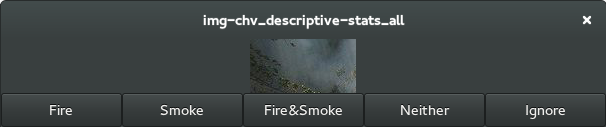
\includegraphics[width=\textwidth]{interview.png}
    \caption{La interfaz gráfica.}
\end{figure}

\subsection{Clases de regiones}
Se utilizan \textbf{5} clases (\refcode{\ExecAll}{exec/DescriptiveStatsAll.hs}):
\begin{enumerate}
    \item \verb|Fire|
    \item \verb|Smoke|
    \item \verb|Fire&Smoke|
    \item \verb|Neither|
    \item \verb|Ignore|
\end{enumerate}

Las instancias etiquetadas con \verb|Ignore| están a la espera de ser removidos.

\subsection{Formato ARFF}

Para la escritura de los datos se utiliza el proyecto \refcode{\WekaData}{WekaData}; el código fuente se incluye en el archivo \verb|WekaData.zip|.

Los adaptadores entre \verb|LearnDataEntry| y \verb|WekaEntry| se encuentran en\\ \refcode{\Weka}{src/ImgCharacteristics/Weka.hs}.

\subsection{Ejecutable}
El proyecto provee varios ejecutables, pero \verb|img-chv_descriptive-stats_all| es el que se usa (\refcode{\ExecAll}{exec/DescriptiveStatsAll.hs}).

Tiene dos modos de uso:
\begin{enumerate}
\item \texttt{img-chv\_descriptive-stats\_all} \textit{images relation target}
\item \texttt{img-chv\_descriptive-stats\_all} \verb|--dir| 
       \textit{directory relation target}
    \begin{itemize}[leftmargin=2cm]
        \item[\textit{images}]   --- enumeración de imágenes;
        \item[\textit{directory}]--- un directorio con imágenes a procesar;
        \item[\textit{relation}] --- nombre de la relación (\verb|@relation|);
        \item[\textit{target}]   --- el archivo \emph{*.arff} a escribir.
    \end{itemize}
\end{enumerate}

\subsection{Compilación}

Requiere:
\begin{itemize}
    \item The Glorious Glasgow Haskell Compilation System (GHC), version 7.10.3.
    \item Common Architecture for Building Applications and Libraries (CABAL),
          version $\geq$ 1.10.
    \item \emph{ghc-gtk3}, version $\geq$ 0.14 (puede ser complicada a compilar).
    \item Proyecto \emph{Nat}.
    \item Proyecto \emph{WekaData}.
\end{itemize}

Las demás dependencias deben ser resueltas por CABAL sin problemas.

\section{Experimentos en Weka}

Para automatizar el proceso de aprendizaje del perceptron, fue creado un pequeño proyecto en Scala. Se aprovecha la facilidad de conexión de aplicaciones de JMV para correr las \emph{evaluaciones} de Weka.

\begin{itemize}
\item Prepara los datos, removiendo las instancias marcadas con la clase 
    \verb|Ignore|.
\item Guarda los reportes de Weka en archivos (por defecto en directorio ``reports'').
\end{itemize}

\medskip
En directorio del proyecto \emph{scripts} se encuentran programas:
\begin{enumerate}
\item \verb|bulkANN.scala| --- fue utilizado para prueba de configuraciones diferentes.
\item \verb|findBestReports.scala| --- selecciona los mejores reportes (por el porcentaje de clasificación correcta).
\item \verb|extractReportsInfo.scala| --- extrae estadísticos desde los reportes y los escribe en archivo.
\end{enumerate}

\medskip
En directorio \verb|octave| se encuentran diferentes utilidades para graficar los comparaciones de los resultados (para Matlab/Octave).

\subsection{Configuraciones de la red}

Fueron realizados experimentos con todas las combinaciones de las siguientes valores:

\begin{center}
\begin{tabular}{l}
\begin{tabular}{|l|l|}
\hline
Variable 					& Valores				\\
\hline
Número de épocas			& 500, 1000, 2000, 3000 \\
``Learning rate ''  		& 0.1, 0.2, 0.5, 0.8 	\\
``Momentum''				& 0.2, 0.5, 0.8 		\\
$1^{\text{ra}}$ capa oculta	& a, t					\\
$2^{\text{da}}$ capa oculta	& 0, a, t				\\
\hline
\end{tabular}\\
\textbf{Total:} 288 combinaciones.
\end{tabular}
\end{center}

$t=\text{núm. de classes} + \text{núm. de attributos} = 56+5=61; a=\dfrac{t}{2}=30$.

%Inicialmente se planeaba hacer pruebas con las combinaciones de las siguientes configuraciones:


\section{Análisis de resultados}

%Fueron recolectadas las estadísticas de las evaluaciones por Weka.
Los mejores resultados fueron demostrados por las \red{siguientes} configuraciones:

\begin{center}
\begin{tabular}{|l|l|l|l|l|l|l|}
\hline
\# épocas & learn. & momenum & $1^{\text{ra}}$ capa & $2^{\text{da}}$ capa & \# correctos & error \\
\hline
\red{?} & \red{?} & \red{?} & \red{?} & \red{?} & \red{?} & \red{?} \\
\hline
\end{tabular}
\end{center}


Para analizar la influencia de diferentes variables sobre la calidad de aprendizaje,
fueron graficados unas proyecciones, los cuales parecen a una histograma, de siguiente manera:

\begin{flalign*}
\text{Sean } &C={c_i} \text{ --- las variables configurables.}\\
			 &E={e_i} \text{ --- las estadísticas para las configuraciones.}\\
			 &D={d_j} \text{ --- los arreglos de configuraciones, tales que}\\
			 &\qquad\begin{aligned}
			 	\forall d_j &\in D  \\
			 	& \forall c_i \in C ~ \exists \text{ un valor } d^c_{ij}
			 		\text{ asociado -- el valor de la variable } c_i\\
			 	&	\qquad \text{ en la configuración } d_j;\\
			 	&\forall e_i \in E ~ \exists \text{ un valor } d^e_{ij}
			 		\text{ asociado -- el valor de la estadística } e_i\\
			 	&	\qquad \text{ en la configuración } d_j.
			 \end{aligned}\\
\end{flalign*}
Una proyección de variables $X,Y \in C$ sobre la estadística $Z \in E$ con operador $op$ es
el conjunto de valores $\{p_{xy}\}$, tales que
\begin{flalign*}
& \forall \text{ único } x \in \text{ valores de } X \\
& \forall \text{ único } y \in \text{ valores de } Y \\
& p_{xy} = op(\{z_{xy}\}) \text{, donde} \\
& \{z_{xy}\} = \left\lbrace d^e_{Zj} ~|~ \forall d_j \in D
	\textbf{ si } d^c_{Xk} = x \wedge d^Y_{Yk} = y \right\rbrace\\		
\end{flalign*}

El operador $op$ puede ser el \emph{promedio}, o valor \emph{máximo/mínimo}, 
o otra función con tipo $\{z\} \mapsto z$.

\begin{figure}[h]
	\centering
	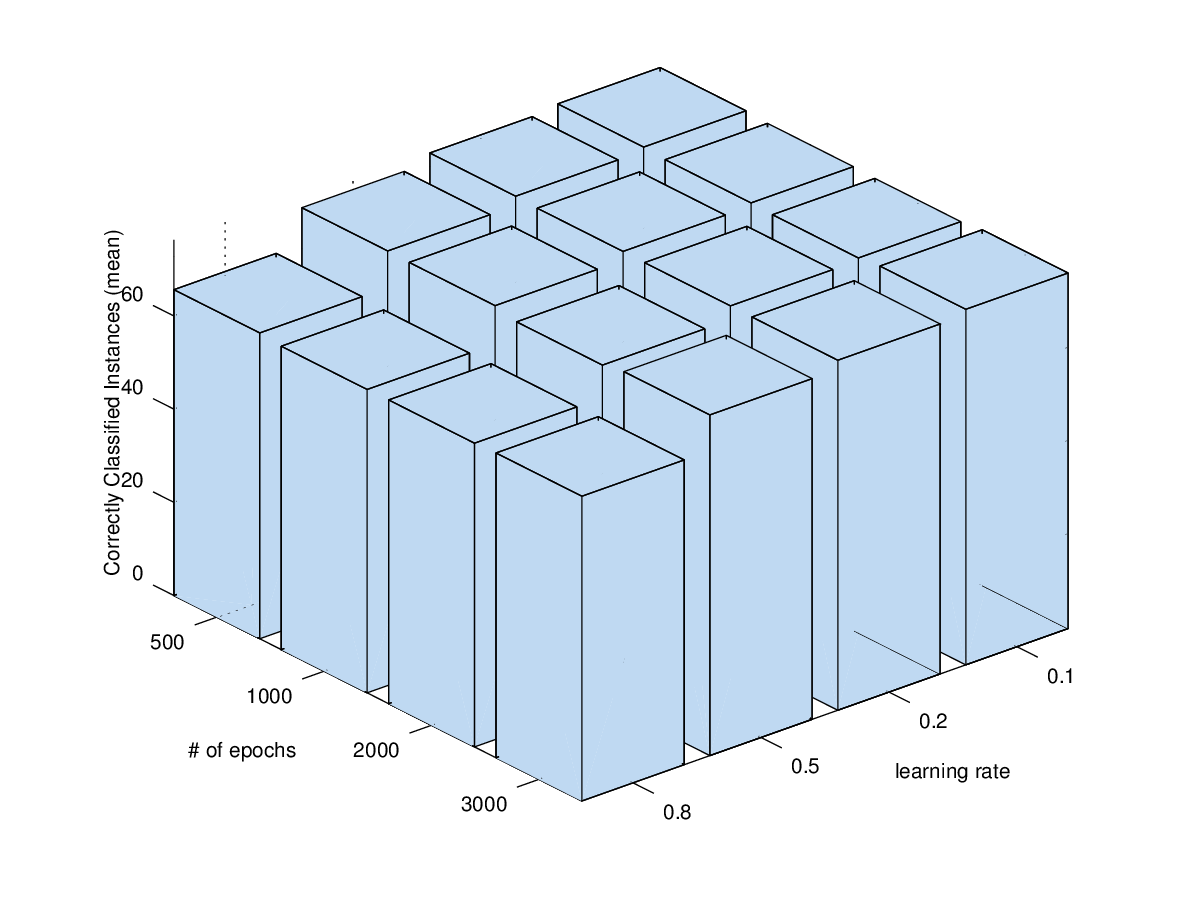
\includegraphics[width=0.49\textwidth]{plots/cmean_NL.png}
	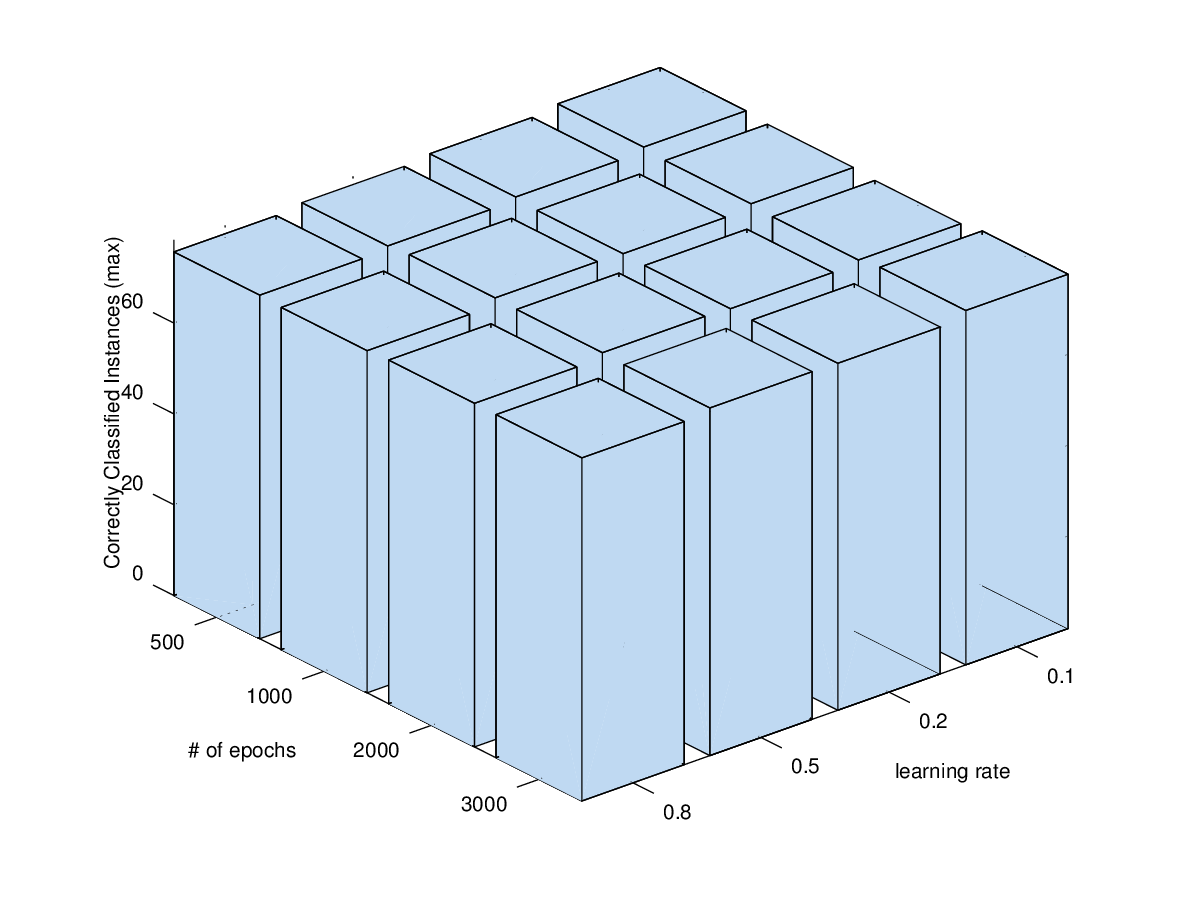
\includegraphics[width=0.49\textwidth]{plots/cmax_NL.png}
	\caption{La proyección del \emph{número de épocas} utilizado y el \emph{``learning rate''} 
			 sobre la \textbf{media} (izquierda) y el \textbf{máximo} (derecha)
			 del \emph{número de instancias correctamente clasificadas}. 
			}
	\label{NL}
\end{figure}


\begin{figure}[h] 
	\centering
	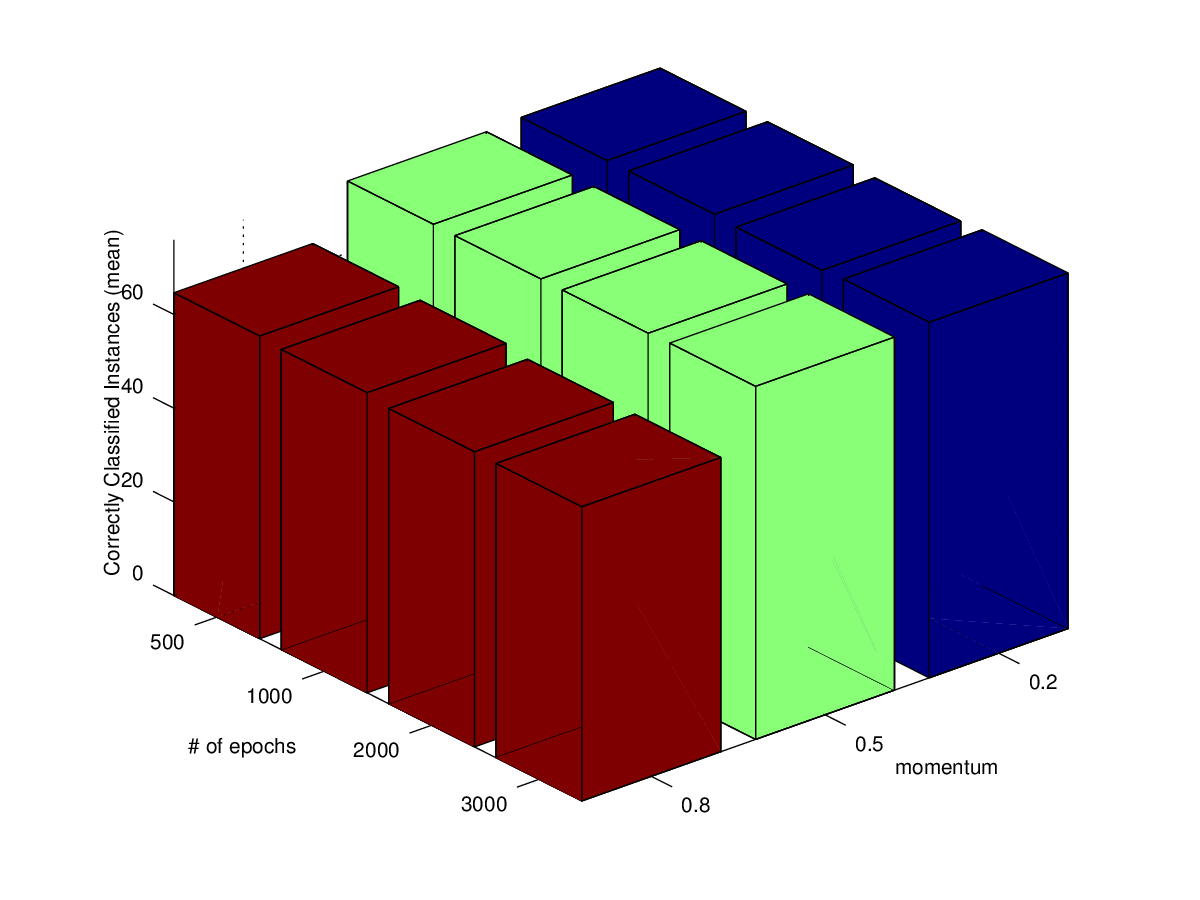
\includegraphics[width=0.49\textwidth]{plots/cmean_NM.png}
	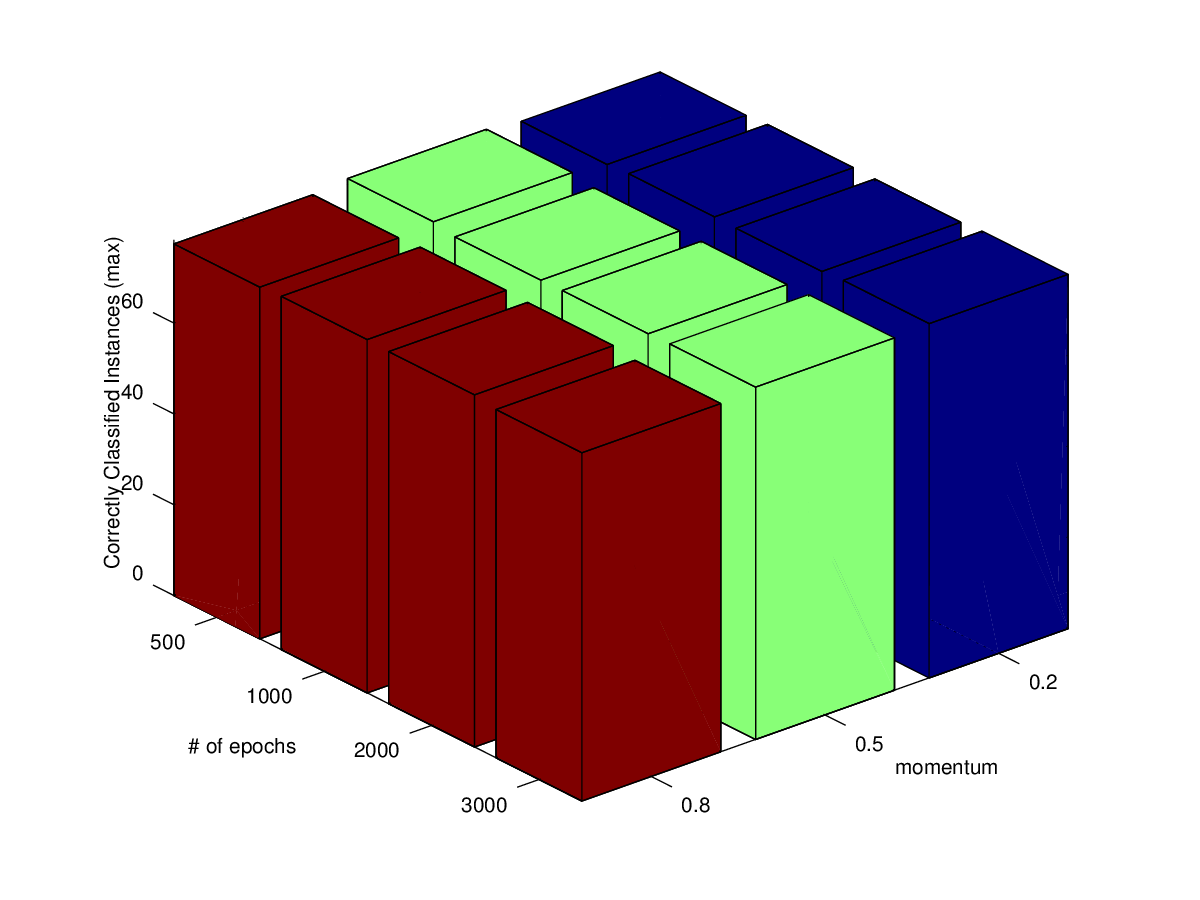
\includegraphics[width=0.49\textwidth]{plots/cmax_NM.png}
	\caption{La proyección del \emph{número de épocas} utilizado y el \emph{``momentum''} 
			 sobre la \textbf{media} (izquierda) y el \textbf{máximo} (derecha)
			 del \emph{número de instancias correctamente clasificadas}. 
			}
	\label{NM}
\end{figure}

\begin{figure}[h]
	\centering
	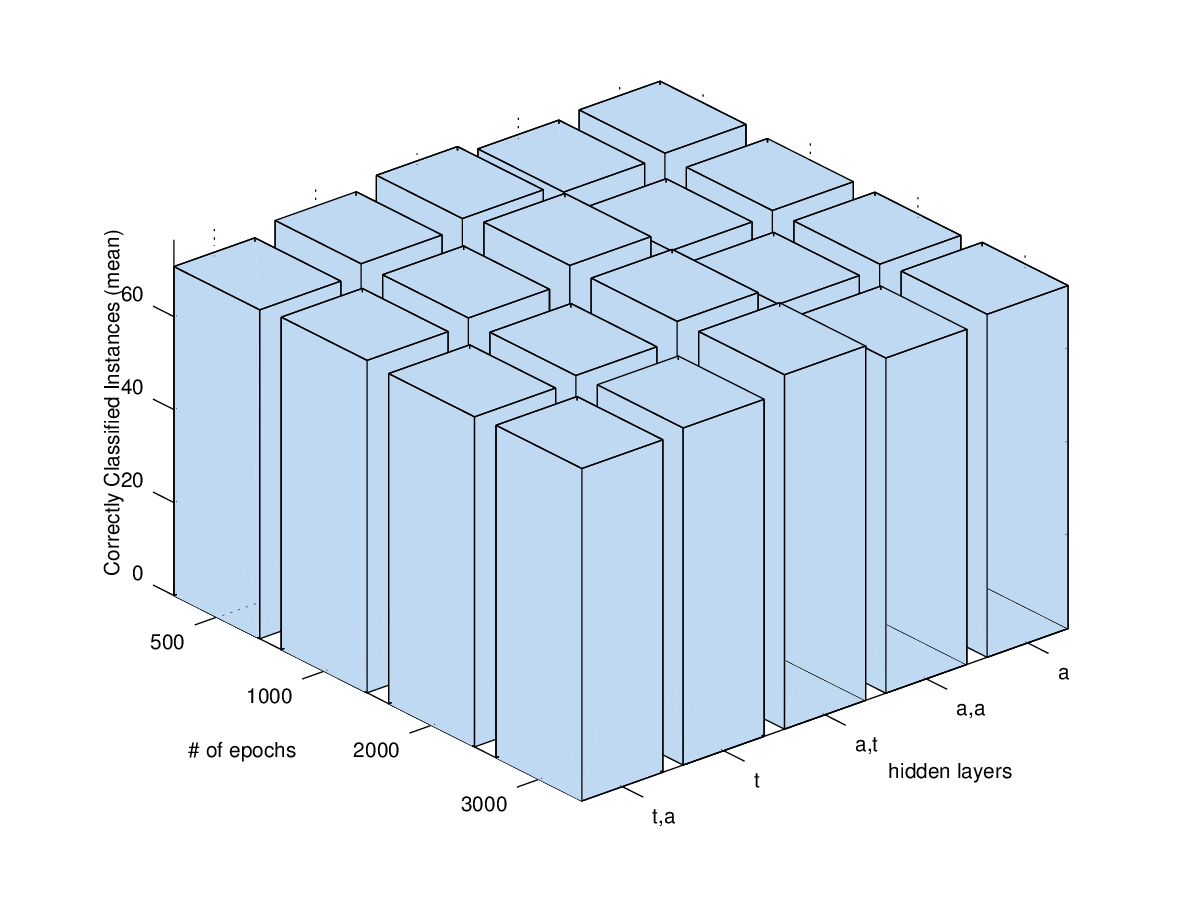
\includegraphics[width=0.49\textwidth]{plots/cmean_NH.png}
	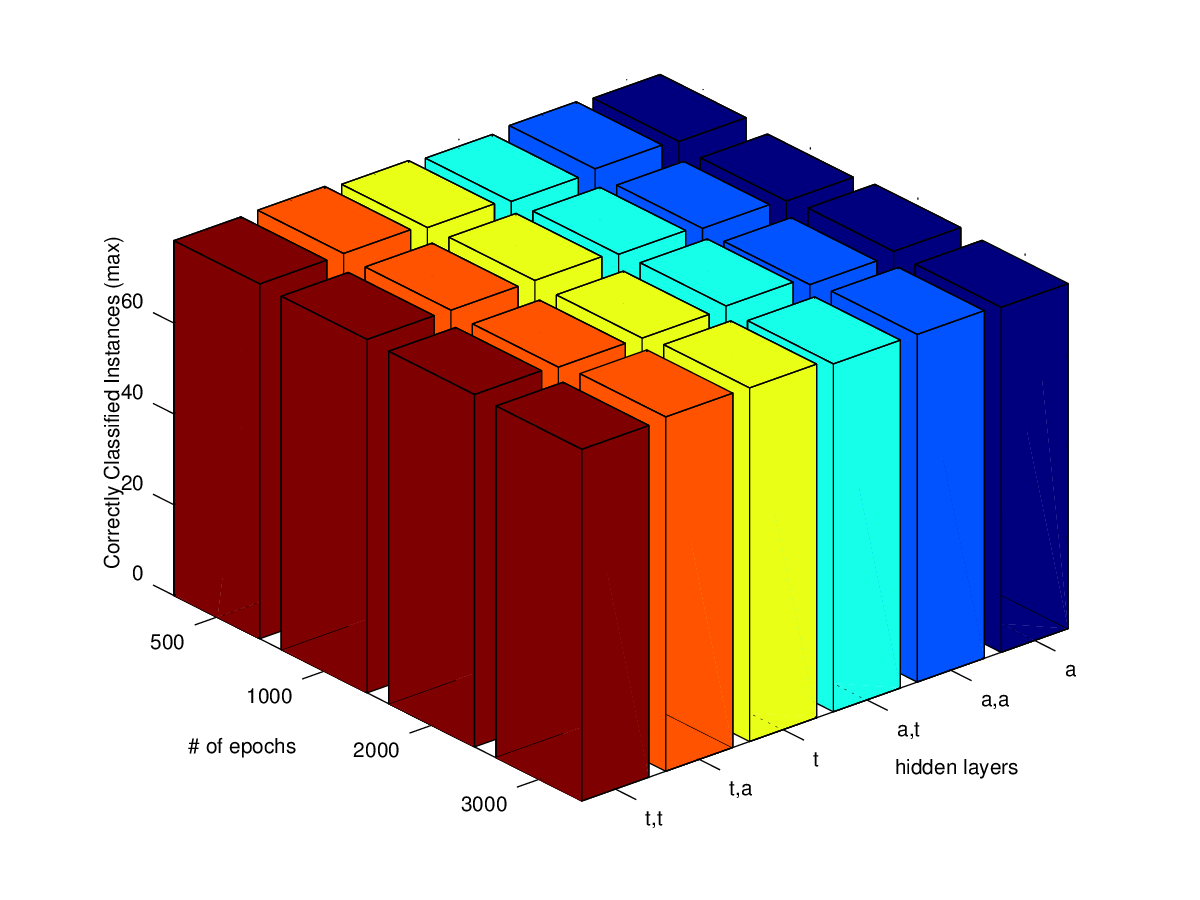
\includegraphics[width=0.49\textwidth]{plots/cmax_NH.png}
	\caption{La proyección del \emph{número de épocas} utilizado y la
			 \emph{configuración de las capas escondidas} 
			 sobre la \textbf{media} (izquierda) y el \textbf{máximo} (derecha)
			 del \emph{número de instancias correctamente clasificadas}. 
			}
	\label{NHc}
\end{figure}
	
\begin{figure}[h] 
	\centering
	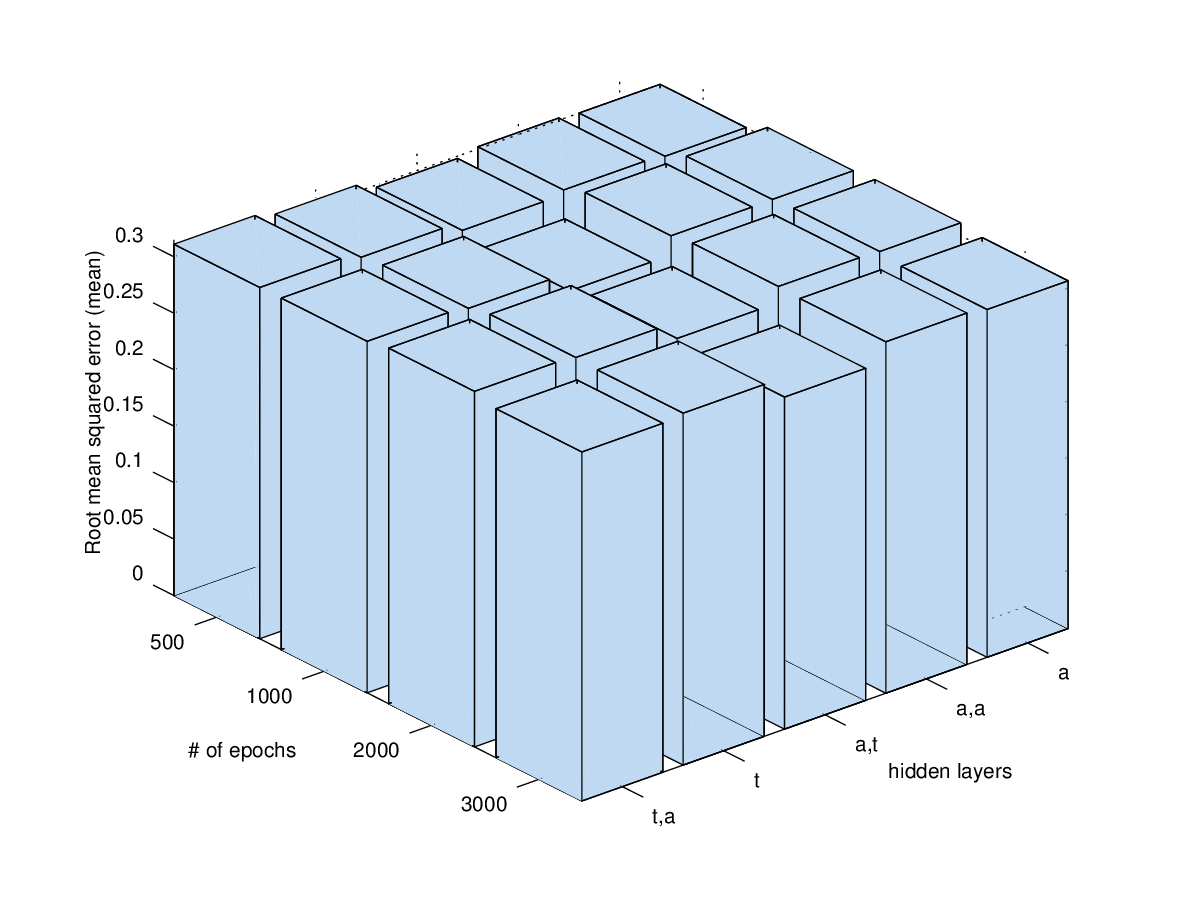
\includegraphics[width=0.49\textwidth]{plots/emean_NH.png}
	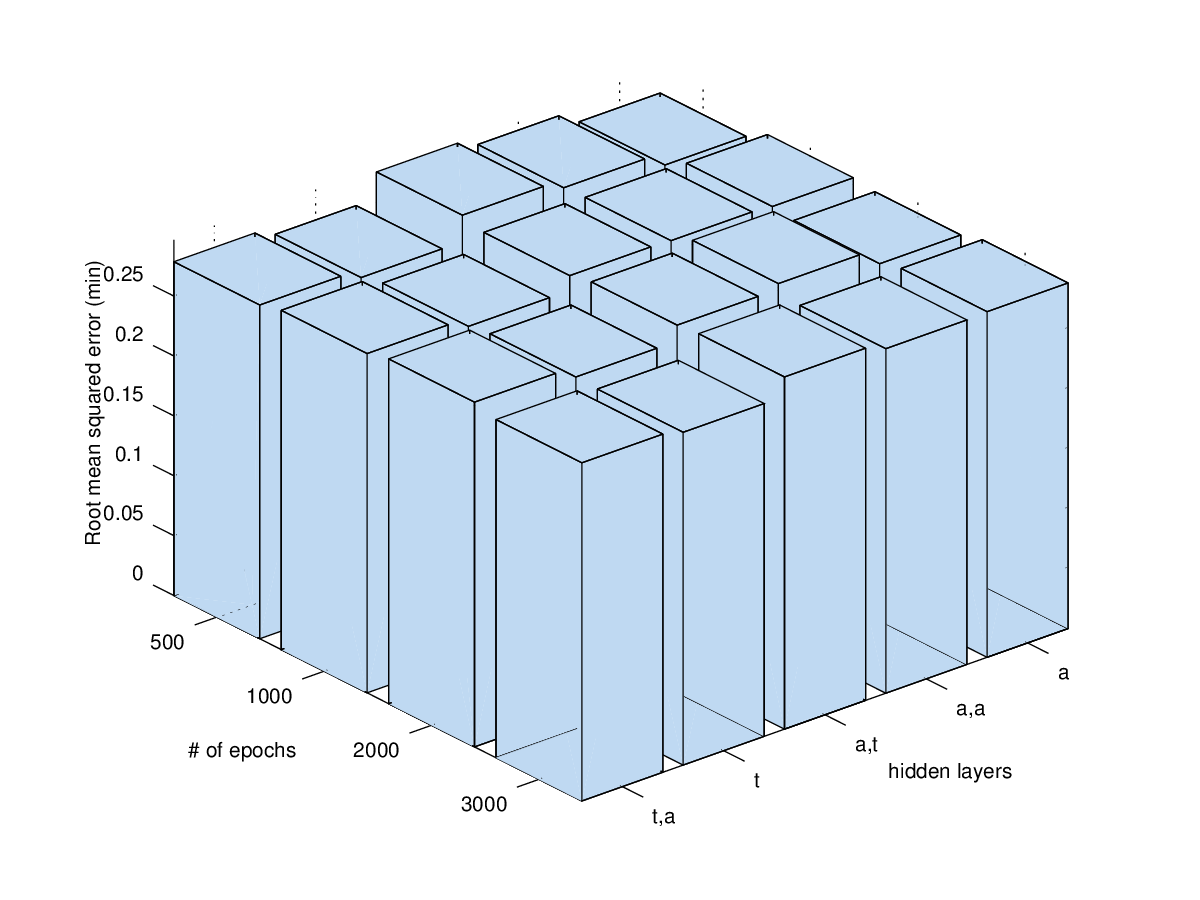
\includegraphics[width=0.49\textwidth]{plots/emin_NH.png}
	\caption{La proyección del \emph{número de épocas} utilizado y la
			 \emph{configuración de las capas escondidas} 
			 sobre la \textbf{media} (izquierda) y el \textbf{mínimo} (derecha)
			 de la \emph{error cuadrática media}. 
			}
	\label{NHe}
\end{figure}	



Se puede ver en la figura \ref{NL} \red{espera todos los datos}.

Se puede ver en la figura \ref{NM} \red{espera todos los datos}.

Se puede ver en la figura \ref{NHc} \red{espera todos los datos}.

Se puede ver que los gráficos en la figura \ref{NHe} es una reflexión \red{(mirror image)} de los gráficos en la figura \ref{NHc}.  \red{Espera todos los datos}.
			 
\end{document}

